\chapter{Project 3: blinking LED}  \label{ch:blink_1}
This project differs from the previous one: in this chapter, the Processing System will be set up without the creation of an example project. It will add more time to the initial configuration, but it is an important step in order to understand what it has to be modified to enable different peripherals within the microprocessor.


\section{Vivado project}
After having created a new Vivado project with the same procedure defined in Chapter \ref{ch:nand_bm}, the constraints file and the source file have to be created. The code is reported in the following:
\begin{itemize}
	\item Constraints file:
		\begin{verbatim}
			set_property BITSTREAM.GENERAL.COMPRESS TRUE [current_design]
			
			#Fan Speed Enable
			set_property PACKAGE_PIN A12 [get_ports {fan_en_b}]
			set_property IOSTANDARD LVCMOS33 [get_ports {fan_en_b}]
			set_property SLEW SLOW [get_ports {fan_en_b}]
			set_property DRIVE 4 [get_ports {fan_en_b}]
			
			#User defined pins
			set_property PACKAGE_PIN F8 [get_ports {uf1}]
			set_property IOSTANDARD LVCMOS18 [get_ports {uf1}]
		\end{verbatim}
	
	\item Source file \#1:
		\begin{verbatim}
			-- Clock Divider
			-- Every match, the output signal is toogled
			-- The output frequency is given by: f_out = f_in / (2*max_val)
			
			library IEEE;
			use IEEE.STD_LOGIC_1164.ALL;
			use IEEE.STD_LOGIC_ARITH.ALL;
			use IEEE.STD_LOGIC_UNSIGNED.ALL;
			
			
			entity prescaler is
			
			    Port ( clk_in, reset   : in STD_LOGIC;
			           clk_out         : out STD_LOGIC);
			
			end prescaler;
			
			
			
			architecture Behavioral of prescaler is
			
			    constant    max_val : integer                       := 500000;  
			    signal      counter : integer range 0 to max_val-1  := 0;
			    signal      tmp     : std_logic                     := '1';
			
			begin
			
			    process(clk_in, reset)
			    begin
			        if reset = '0'
			        then
			            tmp <= '0';
			            counter <= 0;
			        else
			            if rising_edge(clk_in)
			            then
			                if counter = max_val-1  -- Counts from 0 to max_val-1
			                then
			                    counter <= 0;
			                    tmp <= not tmp;
			                else
			                    counter <= counter + 1;
			                end if;
			            end if;
			        end if;
			    end process;
			
			clk_out <= tmp;
			
			end Behavioral;
		\end{verbatim}
	
	\item Source file \#2 (AND gate to be inserted after the clocking wizard):
		\begin{verbatim}
			library IEEE;
			use IEEE.STD_LOGIC_1164.ALL;
			
			entity and_gate is
			
			    Port ( a, b : in STD_LOGIC;
			           y    : out STD_LOGIC);
			end and_gate;
			
			architecture Behavioral of and_gate is
			begin
			
			    y <= a and b;
			
			end Behavioral;
			
		\end{verbatim}
\end{itemize}
After having created all the needed files, it is possible to create the Block Design, that will have the structure defined in \ref{fig:prj3_1}.
\begin{figure}[ht]
	\centering
	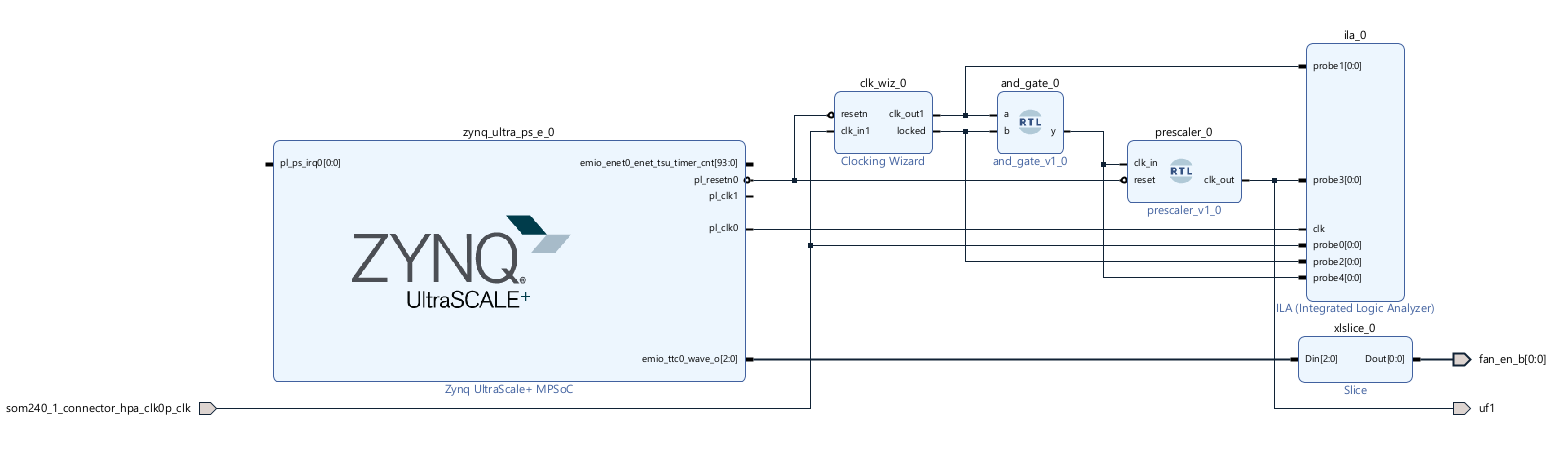
\includegraphics[width=\textwidth]{images/prj3_1}
	\caption{Block Design Layout.}
	\label{fig:prj3_1}
\end{figure} 


\subsection{Block configuration}
The design is composed by few blocks, some of which have already been encountered in the previous implementation. A first, quite useful procedure, is to save the block design of the fan control (example project) and use it as a starting point for new designs. After having opened the fan example, remove both the wrapper and the design file and import the design previously exported (or save the new one with another name). Add and configure the clocking wizard block. Set the reset to be \textbf{active low} and the output clock to be the value that you want (there is, however, a defined range of possible clock frequencies with defined values). For this example the output frequency is set to be $f_{clk-wiz} = 10MHz$. Connect then the and gate, the prescaler and the ILA block as shown in Figure \ref{fig:prj3_1}. Define the output connectors and generate the bitstream. For a more specific configuration, please refer to \href{https://www.hackster.io/LogicTronix/kria-kr260-petalinux-2022-2-gpio-tutorial-9b14bf#toc-vivado-vitis-tool-flow-3}{this page}. Once the bitstream is ready, export the hardware as explained in the previous chapter.




\section{Petalinux project}
The procedure through which the OS is set up and the board booted is the exactly the same defined for the previous project. Also the creation of the bif file and the FPGA programming do not change. Obviously, it will take a while, but at the end the bard will be fully programmed and the led should blink with a frequency of
\begin{equation*}
	f_{blink} = \frac{f_{clk-wiz}}{2 \cdot max\_val} = 10Hz
\end{equation*}



\section{J-TAG debugging}
The main difference between this project and the previous one is the presence of a clock source that will allow for the ILA to trigger and synchronize the displayed signals. After having programmed the FPGA, opened the \textbf{Hardware Manager} and connected the device, Vivado should automatically find the debug-probes file (if not, just re-programm the FPGA). Between the various signals, chose one to be referred as trigger and define the trigger event (equal to a value, rising or falling edge...) and run the trigger event for the ILA core. 
\begin{figure}[ht]
	\centering
	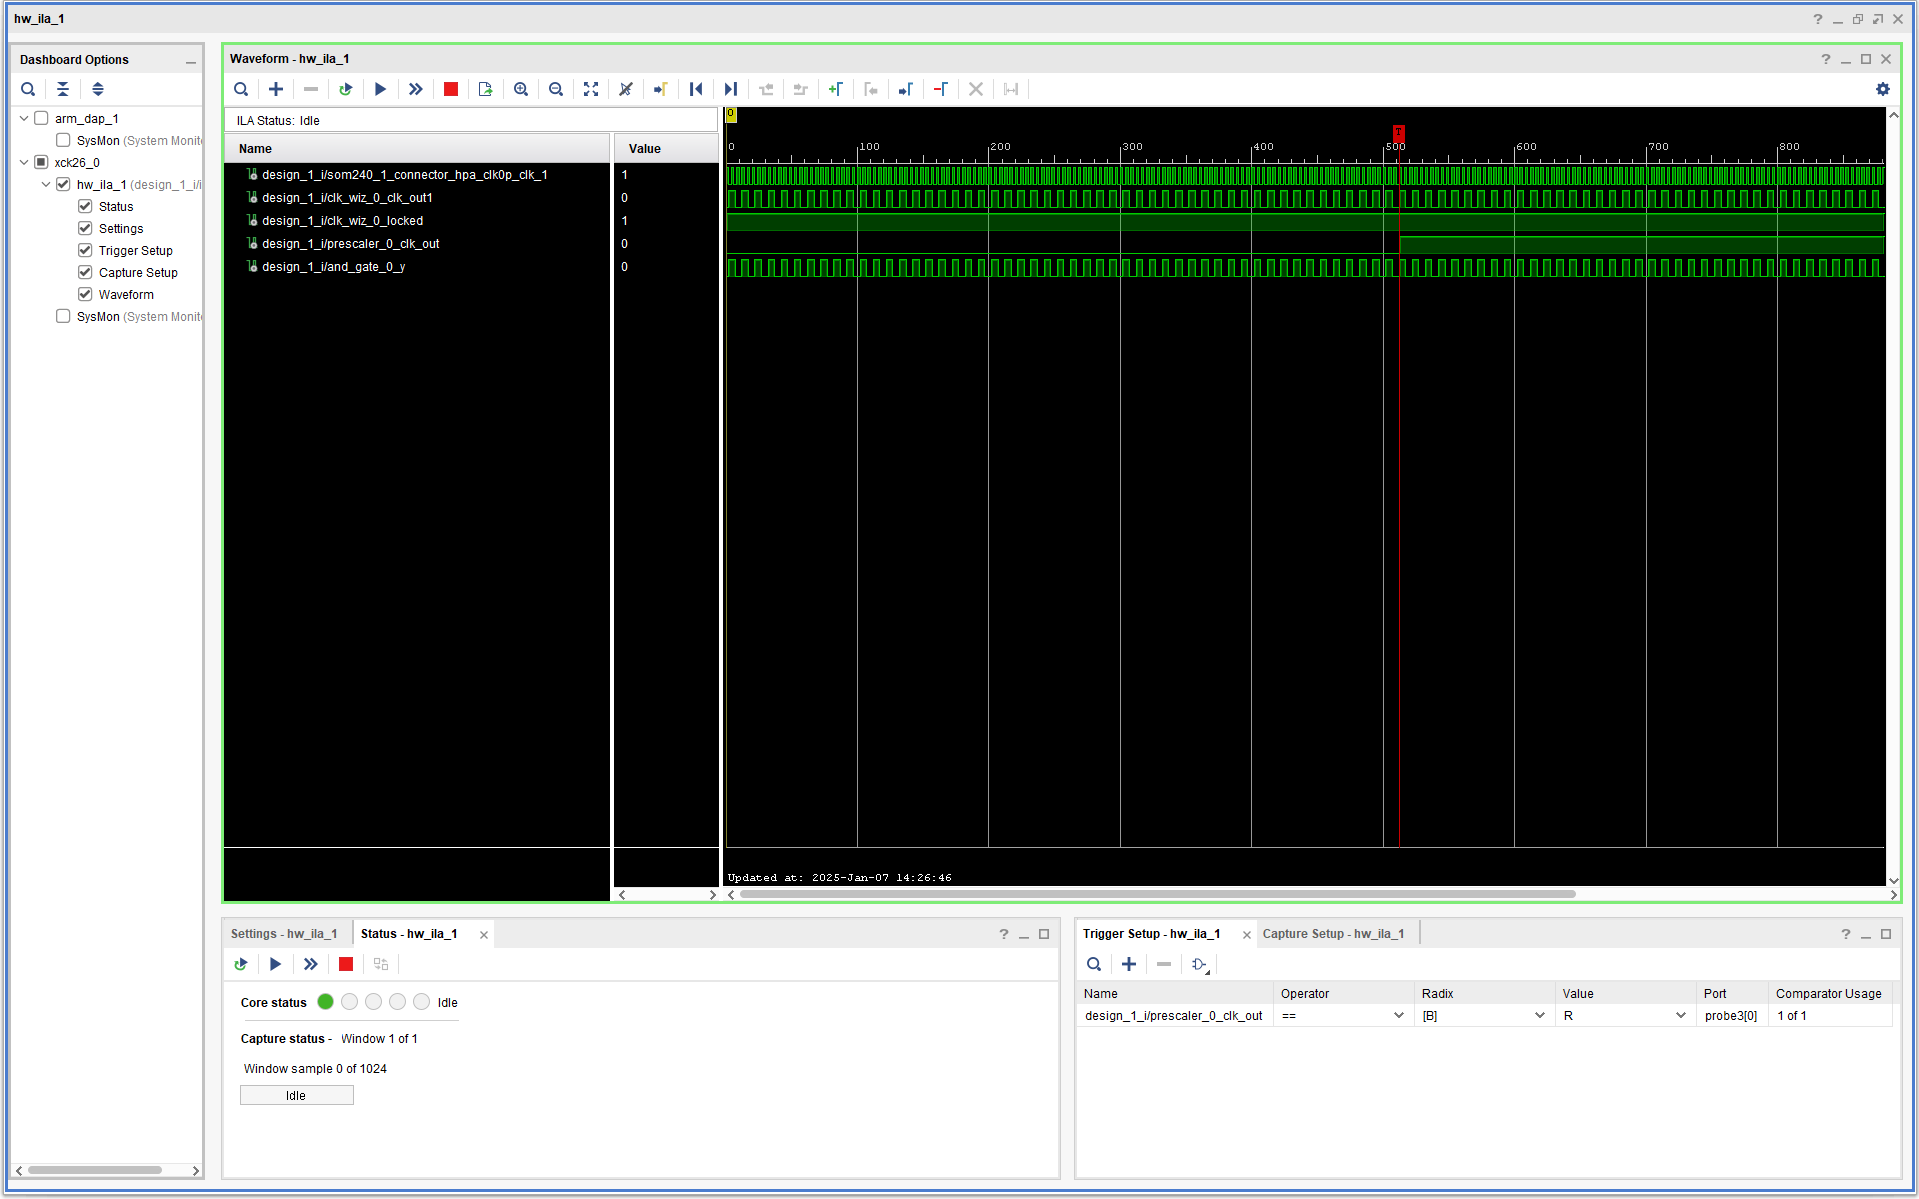
\includegraphics[width=\textwidth]{images/prj3_2}
	\caption{J-Tag debugging with ILA core (triggered on the blinking signal).}
	\label{fig:prj3_2}
\end{figure} 